\documentclass{article}

\usepackage{fullpage}
\usepackage{graphics}

\begin{document}

\begin{center}

{\Large \it CASSBEAM}

\vspace{5pt}

Software for Cassegrain antenna modelling

\vspace{10pt}

{\it Walter Brisken}

\vspace{5pt}

National Radio Astronomy Observatory

\vspace{5 pt}

Version {\bf 1.0} \hspace{0.5in} August 18, 2003
\end{center}

\section{Introduction}

Cassbeam is a Cassegrain antenna ray tracer.  Based on an input text file,
it computes several properties of the antenna including gain,
zenith system temperature, and the beam, in full polarization.  All calculations
are done in the {\it transmit sense} and use reciprocity to relate to the
equivalent receiving system.  

A classical Cassegrain antenna consists of a paraboloidal primary optical 
surface and a hyperboloidal secondary.  This allows a large effective 
focal length to be shortened considerably.  This means that more directive
feeds can be used.  Since wideband feeds tend to have narrower radiation
patterns, the Cassegrain is often a better choice for wide band systems.
A second advantage of Cassegrain systems is that the radiation that
spills over the secondary reaches the cold sky rather than the 290K 
ground.  Shaped Cassegrain systems have primary surfaces that are rotationally
symmetric but no longer paraboloidal.  The secondary is then shaped
as well in order to well define a secondary focus.  Shaping is used to
adjust the amplitude of the illumination across the primary, allowing
for higher aperture efficiency.  An additional deviation from the 
classical Cassigrain is placing the feed off axis and compensating
with an asymmetric secondary.  This is used at the VLA.  It allows a rotation
of the subreflector about the primary's symmetry axis to point the beam 
toward one of six feeds.  Both of these deviations from a classical
Cassegrain are supported.  An example of a offset, shaped Cassegrain antenna
is shown in Fig.~\ref{fig:vlaant}.
Additionally, cassbeam allows deformations, or
``pathologies'' of the optics to be modelled.  Currently this is limited
to rotations and translations of the feed and secondary.  In the future, 
large scale deviations in the primary (such as a misplaced panel) will
likely be supported.

\begin{figure}[h!]
\begin{center}
\resizebox{5in}{!}{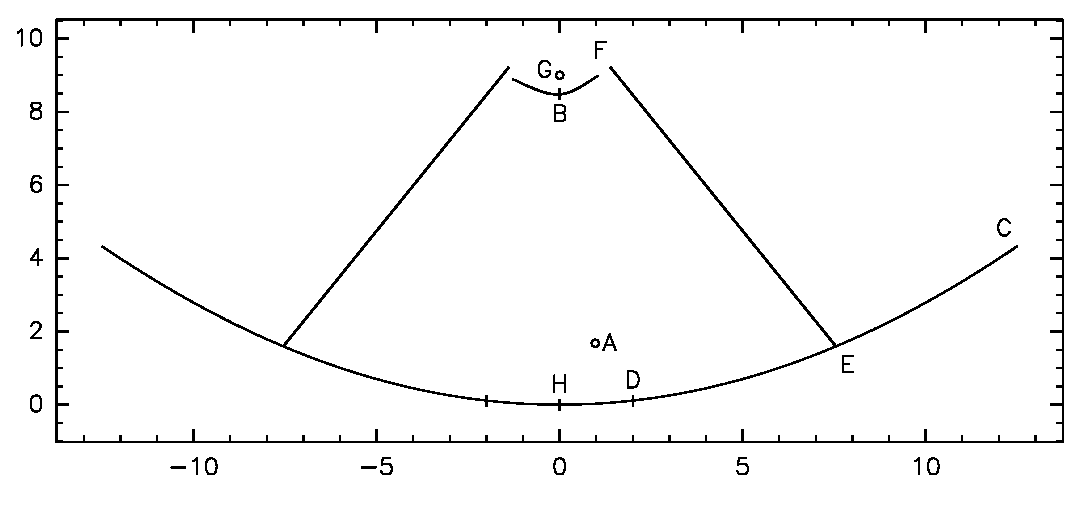
\includegraphics{vlaslice2.eps}}
\begin{tabular}{|l|l|}  \hline
\footnotesize
Point & Coordinates (meters) \\ \hline \hline
A. Feed						& 0.975, 1.676 \\ \hline
B. Intersection of subreflector and primary axis& 0.0, 8.479   \\ \hline
C. Edge of primary				& 12.5, 4.325  \\ \hline
D. Inner edge of paneled primary		& 2.0, 0.112   \\ \hline
E. Base of strut				& 7.550, 1.594 \\ \hline
F. Top of strut					& 1.391, 9.217 \\ \hline
G. Prime focus					& 0.0, 9.0     \\ \hline
H. Vertex of primary				& 0.0, 0.0     \\ \hline
\end{tabular}
\end{center}
\caption{\label{fig:vlaant}
The VLA antenna optics.  This is an example of a shaped, offset Cassegrain.
Coordinates are $x$, $z$.}
\end{figure}

This software is presented to the world under the 
Gnu General Public License (GPL) version 2.0\footnote{See 
{\tt http://www.gnu.org/copyleft/gpl.html} or the LICENSE file included
with the software for more information.}.  The use of this software is at
your risk!  Although this software is thought to produce correct output,
your mileage may vary.

\subsection{Sample use case} \label{sec:use}

Here is a very terse description on how to use cassbeam.  Read this entire
document to understand what is actually happening.  First an input file
must be created.  A sample input file called {\tt X-mid.in}
is shown in Appendix~\ref{apx:sample}.
This file specifies the geometry of the EVLA antenna and has some 
parameters tuned for X-band in particular.  A second file must also 
be created called {\tt vla\_geom} to supply the shape of the primary.  A
portion of this file is shown in Appendix~\ref{apx:vlageom}.
Cassbeam is run simply by supplying the input filename.  A sample 
session is shown in Appendix~\ref{apx:sampout}.
Running this file produces 12 output files that will be explained in
detail in Sec.~\ref{sec:output}.

\subsection{Limitations}

In its current form, cassbeam only computes the properties of Cassegrain
antennas that have a rotationally symmetric primary surface.  The figure of
this primary may be specified as a function of radius.  While all $z(r)$
curves are legal input, pathological surfaces (such as those with negative
$z^\prime(r)$) will either produce non-physical results or will cause
abnormal program termination.  Gregorian geometries, those where the
secondary surface is concave and above the prime focus, will probably produce
correct answers but this geometry is not formally supported.

The number of struts (secondary supports) is currently fixed to be four.
This will likely change with future versions of this software.

Cassbeam works in the optical regime, meaning that the wavelength is assumed
to be infinitesimal.  This allows the use of ray tracing rather than physical
optics, which is much faster and much simpler to implement.  
Antenna geometries with structures with dimensions smaller than about 2 
wavelengths will produce results that deviate from reality, although
tests with $1\,\lambda$ struts show results that are consistent with
a similar simulation using physical optics in Grasp8.  Also optical 
surfaces with sharp edges will likely be treated incorrectly.

\section{Conventions}

In the optics world there are several examples of contradictory conventions
that potentially lead to confusion.  The conventions chosen here aim to be
those most commonly encountered in the radio astronomy community.  In most
cases, these are the same as those used within antenna engineering.  

\subsection{Units}

The metric system is used exclusively over emperial units.  Specifically,
the meter is used as the unit of length, the nanosecond is used as the
unit of time, and all frequencies are measured in GHz.  The user specifies
angles in degrees, although within the software radians are used in all
angular calculations.  All temperatures are in Kelvin.

\subsection{Coordinate systems}

The user must define the coordinates of various antenna components in
{\it antenna coordinates}.  In this right-handed Cartesian coordinate system,
$\hat{z}$ points along the symmetry axis of the antenna, toward the pointing
direction.  Above is always taken to mean ``with greater $z$ value.''  The
$\hat{x}$ direction is taken to be parallel to the ground and $\hat{y}$ is
thus determined by orthogonality.  $\hat{y}$ points away from the ground.
The radial coordinate used to define the shape of the primary is
$r \equiv \sqrt{x^2 + y^2}$.  The origin of the coordinate system is the 
vertex of the primary -- the point on the vertex that intersects the $z$
axis.

\begin{figure}[hb]
\begin{center}
\resizebox{2.5in}{!}{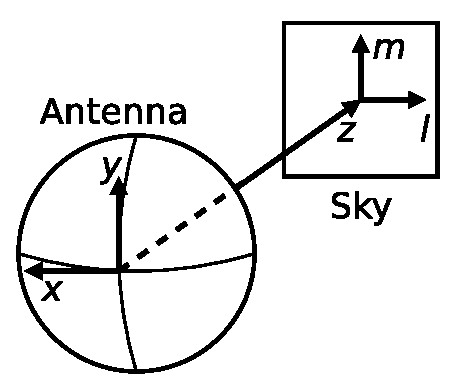
\includegraphics{coords.eps}}
\end{center}
\caption{\label{fig:coords}The antenna and sky coordinate systems.  This
view is from behind the primary surface looking at the sky.}
\end{figure}

The sky coordinate system is a two-dimensional sine-projected angular 
coordinate system used to define the the beam axes.  The sine-projection
comes naturally out of the Fourier transform that relates the aperture
field to the radiation pattern on the sky.  The origin of this coordinate 
system is the pointing direction, $\hat{z}$.  At this point, 
$\hat{l}$ points parallel to $-\hat{x}$ and $\hat{m}$ is parallel to $\hat{y}$.
In other words, $\hat{l}$ points west and $\hat{m}$ points north when the
antenna is pointed at the meridian.

\subsection{Fields}

The vacuum plane wave solutions to Maxwell's equations are harmonic in time.
Internally, complex notation is used in field calculations, which simplifies
notation and allows temporal and spatial evolution of the plane wave fields to 
be expressed with complex exponentials.  The physical
field is the real component of its complex value.  Both sign conventions are 
used for the phase factor.  The convention used by both Jackson and 
Thompson, Moran, and Swenson is used; the evolution of plane wave 
fields is governed by
\begin{equation} \label{eqn:phase}
\vec{E}(\vec{x}, t) = \vec{E}_0 e^{i (\vec{k} \cdot \vec{x} - 2 \pi \nu t)}.
\end{equation}
Note that Born and Wolf use the opposite convention for the phase (and thus
also for circular polarization).
Here $\vec{k}$ is the wave vector (with magnitude $2 \pi / \lambda$) and
$\nu$ is the frequency (cycle rate).  $\vec{E}_0$ is a vector quantity
with magnitude equal to the electric field strength.  The direction of the
vector describes its polarization state.  The electric field is
transverse:
\begin{equation}
\vec{k} \cdot \vec{E}_0 = 0.
\end{equation}
For completeness, it is noted that the magnetic induction is given by
\begin{equation}
\vec{B} = \frac{c}{|k|} \, \vec{k} \times \vec{E}.
\end{equation}

\subsection{Polarization}

A right handed linear polarization coordinate system is used.  The linear
polarization basis unit vectors used, $\mathbf{e}_1$ and $\mathbf{e}_2$, depend
on the direction of propagation, $\mathbf{e}_3$, but always have the following 
orthogonality properties:
\begin{eqnarray}
\mathbf{e}_i^* \cdot \mathbf{e}_j & = & \delta_{ij} \label{eqn:ortho} \\
\mathbf{e}_1 \times \mathbf{e}_2 & = & \mathbf{e}_3
\end{eqnarray}
The IEEE definition of circular polarization is used.  With the above 
phase convention (Eqn.~\ref{eqn:phase}), 
the right and left circular polarization basis vectors are respectively
\begin{eqnarray}
	\mathbf{e}_\mathrm{R} & = & 
		\frac{1}{\sqrt{2}}(\mathbf{e}_1 + i \mathbf{e}_2) \\
	\mathbf{e}_\mathrm{L} & = & 
		\frac{1}{\sqrt{2}}(\mathbf{e}_1 - i \mathbf{e}_2) .
\end{eqnarray}
Note that these two unit vectors and $\mathbf{e}_3$ satisfy the orthogonality
condition of Eqn.~\ref{eqn:ortho}.  A useful property of the circular
polarization basis vectors is that they are eigenvectors of 
$\mathbf{e}_3 \times$ with eigenvalues $-i$ and $i$ for 
$\mathbf{e}_\mathrm{R}$ and $\mathbf{e}_\mathrm{L}$
respectively.  Thus since $\vec{k} = k\, \mathbf{e}_3$,
\begin{eqnarray}
\vec{k} \times \mathbf{e}_\mathrm{R} & = & -ik\, \mathbf{e}_\mathrm{R} 
\label{eqn:ker} \\
\vec{k} \times \mathbf{e}_\mathrm{L} & = &  ik\, \mathbf{e}_\mathrm{L} 
\label{eqn:kel}
\end{eqnarray}

The `1' polarization vector in radio astronomy is often taken to
be that which points toward the meridian (see Fig.~\ref{fig:polcoords}).
Thus for a receiving system, 
$\mathbf{e}_1 \propto \hat{m}$, $\mathbf{e}_2 \propto -\hat{l}$, and
$\mathbf{e}_3 \propto -\hat{z}$.
To avoid confusion $\mathbf{e}_1$ and $\mathbf{e}_2$ are used in lieu
of the explicit Cartesian axes, $\mathbf{e}_x$ and $\mathbf{e}_y$.

\begin{figure}[hb]
\begin{center}
\resizebox{1in}{!}{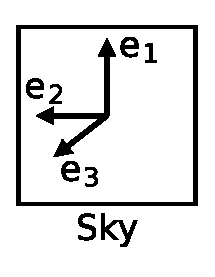
\includegraphics{polcoords.eps}}
\end{center}
\caption{\label{fig:polcoords}The polarization basis vectors.  Note that 
$\mathbf{e}_3$ points out of the page, toward the antenna.}
\end{figure}

\subsection{The Stokes parameters}

The Stokes parameters provide a compact representation of the statistical
properties of the polarization of quasi-monochromatic or broad-band 
radiation.  The 4 parameters are most often labeled $I$, $Q$, $U$, and $V$,
although other conventions, such as $\{s_0, s_1, s_2, s_3\}$ and 
$\{A, B, C, D\}$ also exist.
The Stokes parameters are defined by the following linear polarization products:
\begin{eqnarray}
I & = & \left<E_1^* E_1\right> + \left<E_2^* E_2\right> \\
Q & = & \left<E_1^* E_1\right> - \left<E_2^* E_2\right> \\
U & = & 2 \, \Re \left<E_1^* E_2\right> \\
V & = & 2 \, \Im \left<E_1^* E_2\right> 
\end{eqnarray}
They are equally well defined by circular polarization products:
\begin{eqnarray}
I & = & \left<E_\mathrm{R}^* E_\mathrm{R}\right> + 
	\left<E_\mathrm{L}^* E_\mathrm{L}\right> \\
Q & = & \left<E_\mathrm{R}^* E_\mathrm{R}\right> - 
	\left<E_\mathrm{L}^* E_\mathrm{L}\right> \\
U & = & 2 \, \Re \left<E_\mathrm{R}^* E_\mathrm{L}\right> \\
V & = & 2 \, \Im \left<E_\mathrm{R}^* E_\mathrm{L}\right> 
\end{eqnarray}
In these equations, $E_i \equiv \mathbf{e}_i^* \cdot \vec{E}$ for 
any polarization component $i$ in $\{1, 2, \mathrm{R}, \mathrm{L}\}$.  The
symbols $\Re$ and $\Im$ extract the real and imaginary part of a 
complex number, respectively.

\subsection{Additional terminology}

Here we list some other terminology that will be useful in the following 
sections.  
\begin{description}
\item[aperture plane] The surface in the $x$ -- $y$ plane containing the
rim of the primary.
\item[struts] The secondary supports, or legs.
\end{description}

\section{User reference}

The user provides inputs to cassbeam through an input file.  Additional
options can be passed to cassbeam on the command line.  Based on the arguments
to the {\bf command} parameter, various output files are generated in addition
to the text dumped to the screen.

\subsection{Input files} \label{sec:input}

The main input file consists of a series of lines of the form 
{\it key = value}.  Only one such entry is allowed per line.  The equal 
sign is optional.  The input
files allow comments to be placed within the file.  
All comments begin with {\tt \%}.  This character and any that follow it on
a given line are ignored by cassbeam.  Depending on {\it key}, the {\it value}
may be one of five types: string, integer, double, vector, none.
A string is a sequence of non-whitespace characters {\it not} surrounded 
by quotes of any kind.  A double value is a number that can have a fractional
part.  A vector is a comma-separated list of doubles.  The `none' type expects
no {\it value}.  Below is a list of
the allowed {\it keys} and the type of {\it value} expected.  If the range of
legal values is restricted, the legal range will be contained within brackets.
Note that legal values do not imply a physical system that will generate
meaningful results!  For the vector type, if a certain number of values are
needed, they will be indicated in parentheses.  A required parameter will 
be indicated with a `*'.  It is important to realize that
the secondary optical surface (i.e., the subreflector) is defined based on the
input geometry.  Thus changing the feed placement will change the geometry
of the subreflector!  To change parameters of the telescope without affecting
the shape of the subreflector, set the pathology parameters.  Note that the
order of the parameters does not matter.

\subsubsection{Antenna geometry parameters}

\begin{description}
\item[feed\_x] \ {\it double} \\
The $x$ value of the phase center of the feed.  If no value is provided, 0
is assumed.
\item[feed\_y] \ {\it double} \\
The $y$ value of the phase center of the feed.  If no value is provided, 0
is assumed.
\item[feed\_z] \ {\it double} \\
The $z$ value of the phase center of the feed.  If no value is provided, 0
is assumed.
\item[geom$^*$] \ {\it string} \\
This string points to a disk file containing the primary optical surface
geometry.  This file is a three column ascii text file, each containing
space separated values for $r$, $z$, and $dz/dr$ for the antenna.  There is no
limit (other than your computer's memory) to the number of lines in this file.
It is assumed (but not checked!) that the values of $r$ start at 0 and are
equally spaced.  The radius, $R$, of the primary is given by the value of $r$ in
the last row.  Columns 1 and 2 are in meters, and column 3 is dimensionless.
\item[hole\_radius] \ {\it double} \ [$>$ 0] \\
The radius (in meters) of an unpanelled area at the center of the primary.  If
omitted, no hole will be made.
\item[legapex] \ {\it double} \ [$>$ 0] \\
The $z$ value where the legs (struts) intersect each other.  
Note that the legs might terminate before reaching this point.  The default
value is $1.2*${\bf sub\_h}.
\item[legfoot] \ {\it double} \ [$>$ 0] \\ 
The $r$ value where the legs (struts) intersect the primary surface.  The
default value is half the antenna radius.
\item[legwidth] \ {\it double} \\
The effective width of the legs, used to compute blockage.  Note that currently
a positive value indicates four equally spaced legs with one leg along the
$x$ axis.  If the value is negative, its absolute value is used in
the blockage calculations, but the legs are rotated 45$^{\circ}$.  If this
parameter is not set, or if it is set to 0, then no legs will be generated.
\item[name] \ {\it string} \\
An optional name given to the antenna.  If the name is ``VLBA'', then
the true strut geometry for the VLBA antennas is used rather than 
equispaced struts.
\item[roughness] \ {\it double} \ [$/ge$ 0] \\
The RSS surface roughness in meters.  This number represents the combined
surface error for the primary and secondary.  If no roughness is provided,
the default value of 0 is used.
\item[sub\_h$^*$] \ {\it double} \ [$>$ 0] \\
This value is the $z$ value of the intersection of the subreflector with
the $z$ axis.
\end{description}

\subsubsection{Feed pattern parameters}

Note that either both {\bf feedtaper} and {\bf feedangle} or {\bf feedpattern}
must be provided.

\begin{description}
\item[feedangle] \ {\it double} \ [$>$ 0] \\
Sets the reference angle for the feed taper.
\item[feedpattern] {\it string} \\
The name of the file containing the pattern of the feed.  This file contains
two space-separated columns of numbers: the angle in degrees and the taper
in dB.  The first angle must equal 0, and the angles must be uniformly
spaced.
\item[feedpatternscale] {\it double} \ [$>$ 0] \\
The factor by which to scale the pattern defined in {\bf feedpattern}. 
\item[feedtaper] \ {\it double} \ [$>$ 0] \\
This parameter sets the taper (in dB) of the feed at an angle {\bf feedangle}
from the feed axis to $10^{-\mathbf{feedtaper}/10}$.
\end{description}

\subsubsection{Pathology parameters}

None of the following operations change the shape of the subreflector -- its
geometry is calculated before their application.  Note that displacements
of either the feed or the subreflector result in a rotation of the feed
that corrects for the mispointing caused by the translations.  Rotations
of the feed act in addition to this correction.  Composited rotations (i.e.,
setting {\bf rsub\_x} and {\bf rsub\_y} are both provided), the operations
on the object being rotated proceed in reverse alphabetical order ($z$ 
rotation before $y$ rotation; $y$ rotation before $x$ rotation) regardless
of the order that the parameters are received.

\begin{description}
\item[dfeed\_x] \ {\it double} \\
Displacement of the feed along the $x$ axis.  
\item[dfeed\_y] \ {\it double} \\
Displacement of the feed along the $y$ axis.  
\item[dfeed\_z] \ {\it double} \\
Displacement of the feed along the $z$ axis.  
\item[dsub\_x] \ {\it double} \\
Displacement of the subreflector along the $x$ axis.
\item[dsub\_y] \ {\it double} \\
Displacement of the subreflector along the $y$ axis.
\item[dsub\_z] \ {\it double} \\
Displacement of the subreflector along the $z$ axis.
\item[focus] \ {\it double} \\
Displacement of the feed along the feed axis.  A positive value moves the
feed closer to the subreflector.
\item[rfeed\_x] \ {\it double} \\
Rotation of the feed in degrees about the $x$ axis.  A positive 
value will rotate from the $z$ axis through the $y$ axis.
\item[rfeed\_y] \ {\it double} \\
Rotation of the feed in degrees about the $y$ axis.  A positive 
value will rotate from the $x$ axis through the $z$ axis.
\item[rfeed\_z] \ {\it double} \\
Rotation of the feed in degrees about the $z$ axis.  A positive 
value will rotate from the $y$ axis through the $x$ axis.
\item[rsub\_x] \ {\it double} \\
Rotation of the subreflector in degrees about the $x$ axis.  A positive 
value will rotate from the $z$ axis through the $y$ axis.
\item[rsub\_y] \ {\it double} \\
Rotation of the subreflector in degrees about the $y$ axis.  A positive 
value will rotate from the $x$ axis through the $z$ axis.
\item[rsub\_z] \ {\it double} \\
Rotation of the subreflector in degrees about the $z$ axis.  A positive 
value will rotate from the $y$ axis through the $x$ axis.
\item[subrotpoint] \ {\it vector (1 or 2 or 3)} \\
Defines the point about which the rotation of the subreflector is performed.
The contents of the vector depend on the number of elements are provided:
\begin{enumerate}
\item The $z$ value;
\item The $x$ and $y$ values;
\item The $x$, $y$, and $z$ values.
\end{enumerate}
\end{description}

\subsubsection{Operating condition parameters}

\begin{description}
\item[compute] \ {\it string} [`all' or `none' or combination of 
`a', `j', `p', \& `s'] \\
A string to tell what output to produce.  The string can be `all', `none', 
or a string containing flag characters.  The default value is `all', meaning
produce all possible output.  `none' will produce only messages on the screen
and no output files.  The characters of the general string mean the following:
  \begin{description}
    \item[a] Save the aperture images;
    \item[j] Save the Jones matrices in a table;
    \item[p] Save the parameters;
    \item[s] Save the polarized beams.
  \end{description}
Note that the string is case insensitive.  See Sec.~\ref{sec:output} for
an explanation of the output files.
\item[diffeff] \ {\it double} \\
A user supplied diffraction efficiency.  If none is provided, an internal
algorithm that is not very good is used.  This needs to be upgraded!
\item[freq$^*$] \ {\it double} \ [$>$ 0] \\
The frequency in GHz at which the calculation will be run.
\item[gridsize] \ {\it integer} \ [$\ge$ 32] \\
Specifies a fixed grid size.  If odd, the next even number will be used.
This option overrides any setting of {\bf oversamp} and is the preferred 
method of setting the grid size.  Setting it to a value less than 32 will
result in a grid size of 32.
\item[leggroundscatter] \ {\it double} [$\ge$ 0, $\le$ 1]\\
The fraction of power that scatters off the struts toward the ground.  The
default value is 0.2.
\item[misceff] \ {it double} [$\ge$ 0, $\le$ 1]\\
A factor of the efficiency calculation that contains ``everything else''.  
The user is responsible for choosing a realistic value for this.  A default
of 1 (i.e., 100\%) is assumed if this parameter is not provided.
\item[out] \ {\it string} \\
The prefix for all output files.  The default is {\it cassbeam}.  A dot
will always separate the prefix from any trailing characters.
\item[oversamp] \ {\it double} \ [$>$ 0] \\
One way of specifying the grid size.  This option will make the grid on the
primary fine enough to accommodate 4*{\bf oversamp}*$R/\lambda$ points.  The
default is 1.  Note that vastly ``undersampling'' is fine as the field is
never calculated anywhere between the feed and the aperture plane.  Normally
blockage calculations and constancy of the illumination will dictate the
required sampling.  See {\bf gridsize} for an alternate way of specifying
the grid.  This parameter is ignored if {\bf gridsize} is set.
\item[pixelsperbeam] \ {\it int} [$>$ 0] \\
This is the approximate number of pixels that the core of the beam will
occupy in the output images.
\item[Tground] \ {\it double} \ [$>$ 0] \\
The temperature in Kelvin of the ground.  The default value is 290.
\item[Trec] \ {\it double} \ [$>$ 0] \\
The equivalent temperature of the receiver.  This adds into the system
temperature.  The default value is 50.
\item[Tsky] \ {\it double} \ [$>$ 0] \\
The temperature in Kelvin of the sky.  The default value is 3 for frequencies
over 1~GHz, and $3 \times 10^{-2.5 \nu}$ for frequencies below 1~GHz.
\end{description}

\subsection{Running cassbeam}

Cassbeam is a non-interactive command line program that takes all of its input
from the command line.  Note that this does not preclude someone at a later
date from making a graphical or web front end.  There is one required
argument when running cassbeam -- the input filename that is described
above in Sec/~\ref{sec:input}.  Additional arguments can supplement the
parameters of the input file.  These arguments are passed in the 
same {\it key=value} as required in the input file {\it except} whitespace
is not allowed around the equal sign.  If a parameter appears both
in the input file and the command line, then the value on the command line
supercedes the value on the input file.

\subsection{Output files} \label{sec:output}

Up to 12 output files are generated with version 1.0 of cassbeam depending
on which {\bf compute} options were selected at run time.  These files are
listed below.  The letter in brackets in the section headings indicate which
option is used to enable this file to be written.  All output files begin
with the value of the input parameter{\bf out}.  Currently all output images
are in {\tt .pgm}\footnote{See 
{\tt http://www.die/net/doc/linux/man/man5/pgm.5.html} 
for details on this format.} format, which is a very simple greyscale 
image format supported by most unix-based image viewers.  

\subsubsection{Aperture images [{\bf a}]}

Three images are generated that allow the aperture field to be examined
qualitatively.
If quantitative numbers are needed, the source code should be modified to
export the illumination parameters.
\begin{itemize}
\item {\bf out}{\tt .illumamp.pgm} is a raster image showing the amplitude
of the illumination pattern of the primary.  No blockage is done at this
point.  The scale is linear in flux.
\item {\bf out}{\tt .illumphase.pgm} is a raster image showing the
net phase (pathlength multiplied by wave vector) at each point on the
primary.  A phase gradient is removed.  Portions of the image that correspond
to zero flux have an arbitrary phase.
\item {\bf out}{\tt .illumblock.pgm} is a raster image showing the
blocked portion of the aperture.  White means that this part of the dish is 
experiences either plane wave blockage from the
sky or spherical wave blockage from the feed, and thus does not contribute
to the gain of the antenna.
\end{itemize}

\subsubsection{Jones matrix file [{\bf j}]}

The Jones matrix file, 
{\bf out}{\tt .jones.dat} contains the Jones matrix (see Hamaker et al. 1996 for
details) corresponding to the effect of the antenna on the incoming
radiation as a function of position on the sky.  The file is organized as
an eight column ascii with columns \{$
\Re \, g_\mathrm{RR}, \Im \, g_\mathrm{RR}, 
\Re \, g_\mathrm{LR}, \Im \, g_\mathrm{LR}, 
\Re \, g_\mathrm{RL}, \Im \, g_\mathrm{RL}, 
\Re \, g_\mathrm{LL}, \Im \, g_\mathrm{LL}$\}.  The first row corresponds
to the point on the image with smallese $l$ and $m$.  The rastering
then proceeds first with increasing $l$, and then with increasing $m$.  
There are a total of $n^2$ rows, where $n$ is the smallest odd number
greater than or equal to the {\bf gridsize} used.  The matrices are
rastered on a sine-projected coordinate system tangent to the sky at the
beam center, which corresponds to row number $(n^2+1)/2$.  At the beam center
the pixel scale is given by the output parameter {\bf beampixelscale}, which
is stored in the output file {\bf out}{.params} described below.

\subsubsection{Parameter file [{\bf p}]}

The parameter file, {\bf out}{.params} is an output file in the same format
as the input file, containing all of the input parameters that were 
specified (even if on the command line) as well as many output 
values.  They are:
\begin{description}
\item[Aeff] \ {\it double} \\
The effective area of the antenna [m$^2$].
\item[Aeff\_Tsys] \ {\it double} \\
The effective area of the antenna divided by the system temperature
[m$^2$/K].
\item[ampeff] \ {\it double} \\
The amplitude efficiency, $\eta_\mathrm{I,amp}$.
\item[beampixelscale] \ {\it double} \\
The scale of the generated beam images [deg/pixel].
\item[blockeff] \ {\it double} \\
The blockage efficiency, $\eta_\mathrm{B}$.
\item[diffeff] \ {\it double} \\
The diffraction efficiency, $\eta_\mathrm{D}$.
\item[fwhm\_l] \ {\it double} \\
The full width at half max of the beam in the $l$ direction.
\item[fwhm\_m] \ {\it double} \\
The full width at half max of the beam in the $m$ direction.
\item[gain] \ {\it double} \\
The gain $G$ of the antenna, as defined by Eqn.~\ref{eqn:gain}.
\item[illumeff] \ {\it double} \\
The illumination efficiency, $\eta_\mathrm{I}$.
\item[peaksidelobe] \ {\it double} \\
The directivity of the greatest sidelobe relative to the peak directivity
of the beam.
\item[phaseeff] \ {\it double} \\
The phase efficiency, $\eta_\mathrm{I,phase}$.
\item[point\_l] \ {\it double} \\
The $l$ component of the pointing offset from the $z$ axis 
measured in the image plane.
\item[point\_m] \ {\it double} \\
The $m$ component of the pointing offset from the $z$ axis 
measured in the image plane.
\item[prispilleff] \ {\it double} \\
The primary spillover efficiency, $\eta_\mathrm{S,pri}$.
\item[program] \ {\it string} \\
The name of the program run, which is {\tt cassbeam}.
\item[misceff] \ {\it double} \\
The miscellaneous efficiency, $\eta_\mathrm{M}$.
\item[spilleff] \ {\it double} \\
The spillover efficiency, $\eta_\mathrm{S}$.
\item[subspilleff] \ {\it double} \\
The subreflector spillover efficiency, $\eta_\mathrm{S,sub}$.
\item[surfeff] \ {\it double} \\
The surface efficiency, given by Eqn.~\ref{eqn:surf}.
\item[totaleff] \ {\it double} \\
The total efficiency calculated for the antenna, given by 
Eqn.~\ref{eqn:eff}.
\item[Tsys] \ {\it double} \\
The system temperature calculated with Eqn.~\ref{eqn:tsys}.
\item[version] \ {\it string} \\
The software version number.
\end{description}

\subsubsection{Polarized beam images [{\bf s}]}

With the {\bf s} option, cassbeam will produce 7 images of the beam showing
in the four Stokes parameters the response to an unpolarized source as
a function of the position of the source on the sky.  This information
is derived from the Jones matrices which are saved in
{\bf out}{.jones.dat}.  These images are meant for qualitative inspection.
The Jones matrices contain the formal output.
\begin{itemize}
\item {\bf out}{\tt .I.pgm} Stokes $I$ -- total intensity; 
\item {\bf out}{\tt .Q.pgm} Stokes $Q$ -- excess linear polarization in
$\mathbf{e}_1$ over $\mathbf{e}_2$;
\item {\bf out}{\tt .U.pgm} Stokes $U$ -- excess linear polarization in
$\mathbf{e}_1^\prime$ over $\mathbf{e}_2^\prime$\footnote{
$\mathbf{e}_1^\prime = 1/\sqrt{2}(\mathbf{e}_1 + \mathbf{e}_2)$,
$\mathbf{e}_2^\prime = 1/\sqrt{2}(\mathbf{e}_2 - \mathbf{e}_2)$};
\item {\bf out}{\tt .V.pgm} Stokes $V$ -- excess right circular polarzation
over left circular polarization;
\item {\bf out}{\tt .QI.pgm} The ratio of the Stokes $Q$ image to the 
Stokes $I$ image;
\item {\bf out}{\tt .UI.pgm} The ratio of the Stokes $U$ image to the 
Stokes $I$ image; 
\item {\bf out}{\tt .VI.pgm} The ratio of the Stokes $V$ image to the 
Stokes $I$ image; 
\end{itemize}

\section{Theory of operation}

This section briefly describes how the code works.  Many details are left out.
See the source code if further understanding is needed.

\subsection{Ray tracing} \label{sec:trace}

Ray tracing is used to determine the electric field at each grid point on the
aperture plane.  This is done through a complicated process that will be 
discussed briefly here.  For each grid cell on the primary, the following 
process is followed.

We are interested in calculating the electric field on a uniformly spaced grid
on the aperture plane.  Since the ray may not travel along $\hat{z}$ from the
primary to the aperture plane, some iteration is required.  First the
($x, y$) position of the grid point to be calculated is taken as the starting
point on the primary.  The corresponding $z$ value and the surface normal are
then calculated for that point on the primary.  The virtual ray is then 
reflected off the subreflector.  
It should be noted here that nowhere is the subreflector ever stored as a
rastered surface -- it is recomputed each time it is needed, and this is likely
far more efficient than searching a tabulated surface for an intersection
point.  The subreflector displacement and rotation
are then considered.  A ray is then projected from the feed to this point on
the subreflector.  The process is reversed now that a guess for the 
appropriate subreflector point is made.  A ray is traced from the feed to
this point on the subreflector, reflected toward the primary, and finally
reflected to the aperture plane.  The ($x, y$) value of the intersection
of the ray with the aperture plane is compared with the initial ($x, y$).
An offset is applied to the original value and the iteration continues.  About
3 iterations are sufficient for convergenence, although about 7 are done
in practice.

Once points on both the aperture plane and the primary are known, the final
ray is defined.  Three rays are shot out from a small triangular region of the 
aperture plane and are used to calculate $dP/dA$, the flux through the 
point of interest on the aperture plane.  This value includes the taper of
the feed, the dilution of the beam due to expansion, and the effects of all
the surface shapings.  The length of the ray is then used to derive the
phase of the field on the aperture.  Finally, the two circular polarization
vectors are propagated from the feed.  Reflections obey the proper boundary 
conditions for a conducting surface:
\begin{eqnarray}
E_{\parallel} & = & 0 \\
B_{\perp} & = & 0 
\end{eqnarray}
The electric field, decomposed into a linear polarization basis for each
outgoing circular polarization, is computed on the aperture plane grid.

\subsection{Antenna performance} \label{sec:perf}

The gain, $G$, is calculated by first computing the efficiency, 
$\eta$, and then using 
\begin{equation} \label{eqn:gain}
G = 4 \pi \eta \frac{A}{\lambda^2}.
\end{equation}
Here $\lambda$ is the observing wavelength, and $A$ is the geometric area
of the primary, including any unused portion.  For a circular aperture,
$A = \pi R^2$.  The efficiency is computed by multiplying many factors, each
with its own physical cause:
\begin{equation} \label{eqn:eff}
\eta = \eta_S \, \eta_B \, \eta_{\sigma} \, \eta_I \, \eta_D \, \eta_M
\end{equation}
The meanings and definitions of these factors will be discussed below.

A useful quantity is the total power radiated by the feed, given by
\begin{equation}
P_\mathrm{total} = \int_{4 \pi} \left|E^2(\theta, \phi)\right| \, d \Omega.
\end{equation}
The integral is performed over all $4 \pi$ steradians and 
$\vec{E}(\theta, \phi)$ is the electric field radiated by the feed.
Note that an overall constant factor of $(4 \pi)^{-1}$ is removed from 
this equation to simplify notation.

Of particular importance to radio astronomy is the ratio of gain to 
system temperature.  This is directly related to the on-axis sensitivity 
of the antenna.

\subsubsection{Spillover efficiency, $\eta_\mathrm{S}$}

The spillover efficiency is the fraction of power radiated that ends up
illuminating the primary surface.  For a two reflector system, spillover
can occur at two places: around the subreflector and around the primary.  In
the GO limit, a perfectly aligned Cassegrain antenna will only spill
around the secondary, as any ray hitting the secondary will hit the primary.
For a misaligned system this is no longer strictly true.  The total spillover
efficiency is then a product of the subreflector spillover efficiency,
$\eta_\mathrm{S,sub}$ and that of the primary, $\eta_\mathrm{S,pri}$.
The secondary spillover efficiency is calculated as:
\begin{equation}
\eta_\mathrm{S,sub} = \frac{\int_\mathrm{sub} \left|E^2(\theta, \phi)\right| 
	\, d \Omega}{P_\mathrm{total}}.
\end{equation}
The numerator is the integrated power over the solid angle subtended by the
subreflector.
The total spillover is the fraction of power hitting the primary,
\begin{equation}
\eta_\mathrm{S} = \frac{\int_\mathrm{aper} \left|E^2(x, y)\right| \, dA}
	{P_\mathrm{total}}.
\end{equation}
Here $\vec{E}(x, y)$ is the electric field on the aperture plane and the
integral is performed over the aperture plane.  The contribution to 
spillover due solely to the primary is then determined by
\begin{equation}
\eta_\mathrm{S,pri} = \frac{\eta_\mathrm{S}}{\eta_\mathrm{S,sub}}.
\end{equation}

\subsubsection{Blockage efficiency, $\eta_\mathrm{B}$}

The blockage efficiency can be approximated by examining the projected blocked
area on the aperture plane.   The ray tracing procedure produces a mask
specifies if any portion of a given ray is blocked by a strut, or intersects
the hole in the primary.  Small objects, such as struts, in practice
have a different electrical cross section than geometric cross section, and
this cross section is polarization dependent.  Here we make the ray trace
approximation, which produces reasonably accurate results, except for 
wavelengths that are larger than, or similar in size to, the smallest
significant blocking structures.  The standard expression for blockage
efficiency is used:
\begin{equation}
\eta_\mathrm{B} = 
\frac{\left|\int_\mathrm{aper} \vec{E}(x, y) M(x, y)\, dA\right|^2}
     {\left|\int_\mathrm{aper} \vec{E}(x, y) \, dA\right|^2}.
\end{equation}
Here $M(x, y)$ is the mask expression that has a value of 1 for an 
unblocked location on the aperture, and 0 for a blocked region.  This
formulation allows for partially blocked cells to be numerically
integrated.  

\subsubsection{Surface roughness efficiency, $\eta_\sigma$}

A surface that has roughness will contribute to random scattering and
hence loss of efficiency.  Without derivation we state the surface roughness
efficiency as derived by Ruze (1966):
\begin{equation} \label{eqn:surf}
\eta_\sigma = e^{-\left(\frac{4 \pi \epsilon}{\lambda}\right)^2}.
\end{equation}
The RMS surface error, $\epsilon$, represents contributions from both
the primary and secondary surface; the individual surface errors add in
quadrature.  It should be noted that this equation is strictly true only
for normal incedence.  Deep dishes (i.e., $f/D < 1$) may see deviations from
this estimate since the normal incedence approximation breaks down.

\subsubsection{Illumination efficiency, $\eta_\mathrm{I}$}

An aperture that has uniform amplitude and phase illumination will produce
a beam with the greatest directivity.  The illumination, or aperture, 
efficiency is a measure of the efficiency of a radiating aperture relative
to the uniformly illuminated aperture.  Again without derivation, the
expression used to compute the illumination efficiency is
\begin{equation}
\eta_\mathrm{I} = \frac{\left|\int_\mathrm{aper} \vec{E}(x, y) M(x, y) \, dA
\right|^2}{A_\mathrm{m} \, \int_\mathrm{aper} \left|E^2(x, y)\right|
M^2(x, y) \, dA},
\end{equation}
where $A_\mathrm{m}$ is the {\it masked area},
\begin{equation}
A_\mathrm{m} = \int_\mathrm{aper} M(x, y) \, dA.
\end{equation}

Often the this illumination efficiency is decomposed into factors that
are due to amplitude $\eta_\mathrm{I,amp}$ and phase
$\eta_\mathrm{I,phase}$ with the corresponding values:
\begin{eqnarray}
\eta_\mathrm{I,amp} & = & \frac{\left[\int_\mathrm{aper} \left|E(x, y)\right|
M(x, y) \, dA \right]^2}
{A_\mathrm{m} \, \int_\mathrm{aper} \left|E^2(x, y)\right|
M^2(x, y) \, dA} \\
\eta_\mathrm{I,phase} & = & \frac{\left|\int_\mathrm{aper} \vec{E}(x, y) 
M(x, y) \, dA \right|^2}{\left[\int_\mathrm{aper} \left|E(x, y)\right|
M(x, y) \, dA\right]^2}.
\end{eqnarray}

\subsubsection{Diffraction efficiency, $\eta_\mathrm{D}$}

It should be mentioned immediately that the diffraction efficiency 
calculation is likely wrong.  An equation was emperically derived that 
is probably approximately correct for the VLA.  A scale factor
has been applied that allows antennas with different subreflector
sizes to be used.  This assumes that all diffraction loss is due to the
subreflector, which is likely a good guess.  Note that this efficiency
does not currently depend on taper -- another indication of its inadequacy.

\subsubsection{Miscellaneaous efficiency, $\eta_\mathrm{M}$}

This final efficiency catagory contains everything else.  The user must supply
a value in the input file, otherwise 100\% is assumed.

\subsubsection{System Temperature}

The zenith system temperature is computed by determining the fraction of
transmitted power that would hit the ground, $f_\mathrm{g}$, and sky,
$f_\mathrm{s} \equiv 1-f_\mathrm{g}$, and multiplying each by their
respective temperatures.  The receiver temperature is then added:
\begin{equation} \label{eqn:tsys}
T_\mathrm{sys} = T_\mathrm{rec} + f_\mathrm{g}\,T_\mathrm{g} +
f_\mathrm{s}\,T_\mathrm{s}.
\end{equation}
For a Cassegrain antenna, the fractional power hitting the ground 
is computed as
\begin{equation}
f_\mathrm{g} = (1 - \eta_\mathrm{S,sub}) + f (1 - \eta_\mathrm{B,leg}),
\end{equation}
where $\eta_\mathrm{B,leg}$ is the leg blockage efficiency and $f$ is
a fudge factor.  The first term represents the power that spills over the
primary, and thus hits the ground.  The second term represents the power that
scatters off the struts to the ground.  The fraction of scattered power that
hits the ground is controlled by $f$.  The input parameter to set $f$ is
called {\bf leggroundscatter}.

\subsection{Beam calculation} \label{sec:beam}

Once the aperture plane electric field
is known, the far field radiation pattern can be 
determined.  For each hand of circular polarization, the following operations
are performed.  Fraunhofer diffraction applies as we are interested in the 
far field radiation pattern and the electric field is known over an 
entire surface (it is zero outside the aperture and computed on the aperture).
The radiation at a location $\vec{x}$ is given by
\begin{equation} \label{eqn:fraun}
\vec{E}(\vec{x}) = \frac{i e^{ikr}}{2 \pi r} \, \vec{k} \times
\int_\mathrm{aper} \hat{z} \times \vec{E}(x^\prime, y^\prime) 
\, e^{-i(k_x x^\prime + k_y y^\prime)} \, dA^\prime,
\end{equation}
which is adapted to our application from Eqn.~9.156 of Jackson.  In this
expression, $r = |x|$ and $\vec{k}$ is the wave vector of the transmitted
radiation.  The primed coordinates refer to the coordinates on the
aperture plane; the unprimed coordnates refer to the field test points.
Since the integral in this case is over a uniformly gridded
plane, the integral, $\vec{I}(l, m)$, 
becomes a two-dimensional component-by-component 
forward\footnote{A forward transform as defined in the FFT package called 
FFTW.} FFT
of $\hat{z} \times \vec{E}$.  Here ($l, m$) are the 
sine-projected
angular sky coordinates
equal to ($x/z, y/z$).  This is taken in the limit that $z$ is very large.
In order to reexpress Eqn.~\ref{eqn:fraun} in a circularly 
polarized basis, the radiated electric field is projected on the 
circular polarization basis.  Thus, modulo the complex constant,
the quantities of interest are:
\begin{eqnarray}
E_\mathrm{R}(l, m) & = & \mathbf{e}_\mathrm{R}^* \cdot \vec{k} \times \vec{I} \\
E_\mathrm{L}(l, m) & = & \mathbf{e}_\mathrm{L}^* \cdot \vec{k} \times \vec{I} .
\end{eqnarray}
The vector triple product can be rearranged, and Eqns.~\ref{eqn:ker} and
\ref{eqn:kel} can be used simplfiy these to
\begin{eqnarray}
E_\mathrm{R}(l, m) & = & ik\,\mathbf{e}_\mathrm{R}^* \cdot \vec{I} \\
E_\mathrm{L}(l, m) & = & -ik\,\mathbf{e}_\mathrm{L}^* \cdot \vec{I}.
\end{eqnarray}

\appendix
\section{Input file} \label{apx:sample}

This appendix contains a sample input file for cassbeam.  This file
describes in detail the geometry for an EVLA antenna at 10.0~GHz.  Note
that this may not in fact truly represent the geometry of the EVLA -- it 
is meant as an example only.

\begin{verbatim}
# X-mid.in  -- an input file for simulating mid X-band with EVLA
name = EVLA
# EVLA geometry
sub_h = 8.47852      # meters from vertex to subreflector 
feed_x = 0.97536     # meters from optic axis to feed ring 
feed_y = 0.0         # Note that the position on the feed ring is not right
feed_z = 1.67640     # height of feed ring from vertex 
geom = vla_geom      # file containing the primary surface profile
feedtaper = 13.0     # dB below peak
feedthetamax = 9.26  # degrees
legwidth = 0.27      # meters wide
legfoot = 7.55       # meters from optic axis at dish
legapex = 10.93876   # meters above vertex
hole_radius = 2.0    # meters -- radius of unpanelled area
roughness=0.00035    # meters RMS error of combined surfaces
# Abnormalities	specific to mid-X band
focus=-0.289         # the phase center is below the feed circle
dsub_z=-0.005        # the subreflector is moved to compensate for this
# Running parameters
freq = 10.0          # GHz
gridsize = 100       # pixels on a side
Trec=18
out = X-mid
\end{verbatim}

\section{Primary profile input file} \label{apx:vlageom}

This appendix contains a sample file containing the profile of the primary
surface.  Note that only a portion of the file is shown.  1240 lines have been
omitted and replaced with elipses.  The first column is the radial coordinate
$r$ in meters.  The second column is the axial coordinate $z$, also in meters.
The third column is the local derivative $dz/dr$.

\begin{verbatim}
0.000000 0.000000 0.000000
0.010000 0.000003 0.000561
0.020000 0.000011 0.001122
0.030000 0.000025 0.001683
0.040000 0.000045 0.002244
0.050000 0.000070 0.002805
0.060000 0.000101 0.003366
0.070000 0.000137 0.003927
.
.
.
12.480000 4.311402 0.671823
12.490000 4.318122 0.672216
12.500000 4.324847 0.672607
\end{verbatim}

\section{Sample session} \label{apx:sampout}

This appendix contains an example of the text output when running cassbeam.

\begin{verbatim}
parallax<365>% cassbeam X-mid.in
Antenna: VLA  0x80aba60
  freq    = 10.000000 GHz  lambda = 0.029979 m
  Tsky    = 3.000000 K Tground = 290.000000 K Trec = 18.000000 K
  dir     = -0.000000e+00 0.000000e+00 1.000000e+00
  feeddir = -0.142041, 0.000000, 0.989861
  ftaper  = 13.000000
  thmax   = 9.260000

Pathology: 0x80ac608
  subrot = Matrix (3 by 3)
    1.000000     0.000000     0.000000 
    0.000000     1.000000     0.000000 
    0.000000     0.000000     1.000000 
  feedrot = Matrix (3 by 3)
    1.000000     0.000000     0.000000 
    0.000000     1.000000     0.000000 
    0.000000     0.000000     1.000000 
  subshift = 0.000000e+00 0.000000e+00 -5.000000e-03
  subrotpoint = 0.000000e+00 0.000000e+00 8.478520e+00
  feedshift = 0.000000e+00 0.000000e+00 0.000000e+00

Output: 0x80ae2f8
  Spillover eff = 0.922563
    primary     = 0.997158
    subreflector= 0.925193
  Blockage eff  = 0.857039
  Surface eff   = 0.978706
  Illum eff     = 0.993388
    phase eff   = 0.994786
    amp eff     = 0.998595
  Diffract eff  = 0.977420
  Misc eff      = 1.000000
  Total eff     = 0.751363
  Gain          = 5156891.55  =  67.12 dBi
  Tsys          = 24.419 K
    ground      =  3.454 K
    sky         =  2.964 K
    rec         = 18.000 K
  Aeff          = 368.824311 m^2
  Aeff/Tsys     = 15.104166 m^2/K
  l beamshift   = -0.000115 deg
  m beamshift   = -0.000000 deg
  l beam FWHM   = 0.070499 deg
  m beam FWHM   = 0.070676 deg
  Peak sidelobe = 0.039489 = -14.035194 dB

Output image scale is 0.002147 deg/pixel
\end{verbatim}

\section{References}

\noindent
Born, M. \& Wolf, E., ``Principles of Optics: Electromagnetic Theory of
Propagation, Interference and Diffraction of Light,'' 6th edition, FIXME...

\vspace{10pt}

\noindent
Frigo, M., \& Johnson, S. G., ``The Fastest Fourier Transform in the West,'' 
{\tt http://www.fftw.org/}.

\vspace{10pt}

\noindent
Hamaker, J. P., Bregman, J. D., \& Sault, R. J., ``Understanding Radio
Polarimetry, I. Mathematical Foundations,'' 1996,
Astronomy \& Astrophysics Supplemental Series, 117, pp. 137-147.

\vspace{10pt}

\noindent
Jackson, J. D., ``Classical Electrodynamics,'' 2nd edition, 1975, Wiley.

\vspace{10pt}

\noindent
Ruze, J., ``Antenna Tolerance Theory -- A Review,'' 1966, Proceedings of IEEE,
vol. 54, no. 4.

\vspace{10pt}

\noindent
Thompson, A. R., Moran, J. M., \& Swenson, G. W. Jr., ``Interferometry and
Synthesis in Radio Astronomy,'' 2nd edition, 2001, Wiley Interscience.

\end{document}
